\documentclass[conference]{IEEEtran}
\IEEEoverridecommandlockouts
% The preceding line is only needed to identify funding in the first footnote. If that is unneeded, please comment it out.
\usepackage{cite}
\usepackage{amsmath,amssymb,amsfonts}
\usepackage{algorithmic}
\usepackage{graphicx}
\usepackage{textcomp}
\usepackage{xcolor}
\usepackage{multirow}
\usepackage[capitalise]{cleveref}
\crefname{section}{Sec.\@}{Sec.\@}%
\crefname{subsection}{Sec.\@}{Sec.\@}%
\crefname{subsubsection}{Sec.\@}{Sec.\@}%

\def\BibTeX{{\rm B\kern-.05em{\sc i\kern-.025em b}\kern-.08em
    T\kern-.1667em\lower.7ex\hbox{E}\kern-.125emX}}
\begin{document}

\title{Energy Efficient Scheduling for Mobile Asymmetric Multicore Processors}


%\author{\IEEEauthorblockN{1\textsuperscript{st} Christopher Brown}
%\IEEEauthorblockA{\textit{School of Computer Science} \\
%\textit{University of St Andrews}\\
%St Andrews, Scotland \\
%email address or ORCID}
%\and
%\IEEEauthorblockN{2\textsuperscript{nd} Given Name Surname}
%\IEEEauthorblockA{\textit{dept. name of organization (of Aff.)} \\
%\textit{name of organization (of Aff.)}\\
%City, Country \\
%email address or ORCID}
%\and
%\IEEEauthorblockN{3\textsuperscript{rd} Given Name Surname}
%\IEEEauthorblockA{\textit{dept. name of organization (of Aff.)} \\
%\textit{name of organization (of Aff.)}\\
%City, Country \\
%email address or ORCID}
%\and
%\IEEEauthorblockN{4\textsuperscript{th} Given Name Surname}
%\IEEEauthorblockA{\textit{dept. name of organization (of Aff.)} \\
%\textit{name of organization (of Aff.)}\\
%City, Country \\
%email address or ORCID}
%\and
%\IEEEauthorblockN{5\textsuperscript{th} Given Name Surname}
%\IEEEauthorblockA{\textit{dept. name of organization (of Aff.)} \\
%\textit{name of organization (of Aff.)}\\
%City, Country \\
%email address or ORCID}
%\and
%\IEEEauthorblockN{6\textsuperscript{th} Given Name Surname}
%\IEEEauthorblockA{\textit{dept. name of organization (of Aff.)} \\
%\textit{name of organization (of Aff.)}\\
%City, Country \\
%email address or ORCID}
%}

\maketitle

\begin{abstract}
We present a novel adaptive technique for dynamic runtime configuration of asymmetric multicore processors in mobile devices. Our technique measures the current system load of a mobile device, estimates the number of cores of each type (e.g.~high-performance, energy-efficient and balanced cores) and their frequencies that are required for achieving a desired degree of quality of service and then reconfifures the processor to switch off unneeded cores in order to save energy. A near optimal configuration for the current system load is derived using a regression-based machine learning model. We evaluate our technique on a set of novel representative workloads for mobile devices, simulating typical day-to-day user activity on these devices, and demonstrate a reduction in energy consumption of XX\% compared to the default Android operating system scheduler. We also demonstrate that, with the reduced number of cores used,  we are able to achieve the quality-of-service that is within XX\% of the perofrmance under full system.
\end{abstract}

\begin{IEEEkeywords}
Asymmetric multicore processors, Android phones, Energy efficiency, Task scheduling, Dynamic core switching
\end{IEEEkeywords}

\section{Introduction}
Modern mobile devices, such as mobile phones and tablets, are built around modern multi-core processors, and are typically powerful enough to execute tasks that have, until recently, been reserved only for high-end high-performance systems (e.g.~AI on the edge). These high-performance mobile systems, however, come with a cost, as more power brings higher energy consumption and the need for frequent recharging: resulting in inconvenience for the users and harm to the environment. Moreover, the types of processors that drive modern mobile devices are often \emph{asymmetric}, including cores with different power and energy efficiency profiles. For example, the latest generation of Google Pixel mobile phones include an 8-core processor which has 4 \emph{small} cores (the least powerful, but the most energy efficient), 2 \emph{medium} cores (representing a balance between power and energy consumption), and 2 \emph{large} cores (the most powerful, but the least energy efficient). Each of these cores can individually be powered on and off, and their frequency can be adapted during the device operation to increase/decrease processing power and energy consumption. However, the Android operating system \emph{lacks proper support for this feature}, especially support for the adaptation of the cores' configuration to dynamic changes in workload of the system. Furthermore, the Android operating system by default never fully powers off the cores, and thus does not allow them to enter fully energy-efficient state, where these cores really use a minimal amount of energy (CHECK THIS!).

In this paper, we present a novel adaptive technique for the dynamic runtime adaptation of the processor configuration, including the number, frequency and profile of cores switched on. Our technique measures the system load, in terms of the utilisation of the complete system. Based on this, our scheduler decides which cores should be powered on, and at what frequency they should operate at. The remaining cores are powered off (or, in more technical terms, prevented from having any threads scheduled on them, which allows them to go into the deep-sleep state, thus making them effectively powered off).  Our goal with this is to ensure that the energy consumption is minimised while there are still enough resources to meet the minimum requirements in terms of Quality of Service. This is achieved using a regression-based machine learning model for deriving a near-optimal processor configuration (in terms of energy consumption) based on the current workload. We provide an implementation of the technique for processor configuration based on this model in the Android OS kernel. We also evaluate our technique on a set of representative scenarios that model realistic use of mobile devices in everyday life. Using our technique, we have achieved a reduction of 68\% in energy consumption for our scenarios, compared to the default Android OS kernel scheduler. We also show that the reduction in Quality-of-Service when using a reduced set of processor resources using our technique is acceptable (XX\% at most), taking into account the achieved energy saving. 
%
In this paper, we make the following novel research contributions:
\begin{enumerate}
\item We introduce a novel regression-based model for deriving a near-optimal configuration of heterogeneous multicore processors, based on the current system load;
\item We provide an implementation of an Android kernel module, based on the regression model, that dynamically re-configures the processor cores, switching the cores on and off, and changing the frequency of the active ones, during a mobile device operation;
\item We provide a set of representative mobile benchmarks that model the realistic usage of mobile devices by standard users;
\item We evaluate our algorithm on the developed benchmarks, on a Google Pixel 6a mobile device, achieving XX.
\end{enumerate}

\section{Motivation}
\label{sec:motivation}

\begin{table}[ht]
\renewcommand{\arraystretch}{1.3}
\caption{Device and OS specifications for the Google Pixel 6a Android mobile device used for the evaluation results.}
\label{tab:devicespecs}
\centering
%\resizebox{8cm}{!}{%
\begin{tabular}{|c|c|}
\hline 
\textbf{Category} & \textbf{Pixel 6a} \\ % & \textbf{Pixel 7} \\
\hline
      OS version & Android 13/Lineage OS 1.20 \\
      Kernel version & Linux version 5.10.157-g69987828e43a \\
      Architecture & AArch64 \\
      Endianness & Little endian \\
      Number of CPUs & 8  \\
      CPU frequencies & 4x1.8GHz, 2x2.25GHz, 2x2.8GHz \\
      RAM & 6GB  \\
      \hline 
\end{tabular}
%}
\end{table}

In this section, we focus on an example mobile device that is used throughout the context of this paper - a Google Pixel 6a mobile phone,  containing an octa-core CPU that has 4 (\emph{large}) Cortex X1 cores running at 2.8Ghz, 2 (\emph{medium}) Cortex A75 cores running at 2.25 GHz and 2 (\emph{small}) Cortex A55 cores running at 1.55 GHz (the hardware of the 6a  device is summarised in~\cref{tab:devicespecs}). Each of these core types has a different power-performance trade-off, with smaller cores offering a significantly more efficient power profile at the expense of slower performance, and larger cores offering faster performance at the expense of more inefficient power profiles.

\begin{table}
\renewcommand{\arraystretch}{1.3}
\caption{Activity of the cores of Google Pixel 6a phone when running a web browser benchmark}
\label{tab:actweb}
\centering
\begin{tabular}{|c|c|c|c|c|}
\hline
\textbf{CPU ID} & \textbf{Num wkps} & \textbf{Avg wkp} &  \textbf{Avg sleep} \\
\hline
      3 &  960 &     0.23ms &        0.81ms \\      
      0 &    918 &      0.28ms &           0.80ms \\
      1 &    879 &       0.27ms &          0.87ms \\
      4 &    282 &       0.15ms &           3.39ms \\
      2 &  837 &       0.29ms &          0.90ms \\
      5 &    242 &       0.12ms &             3.96ms \\
      7 &     32 &       0.22ms &            31.55ms \\
      6 &     21 &       0.11ms &           46.95ms \\ 
      \hline
\end{tabular}
\end{table}

Consider one of the typical scenarios of the practical use of a mobile phone, where a user interactively runs a web browser in the foreground, while some other tasks (e.g.~a mail client checking for new emails, a messaging app checking for new messages, or various system services such as network daemons) are running in the background. Many of these background tasks will wake up periodically (typically at different times) and run for a very brief time before getting suspended. Since each task is required to be executed on one of the CPU cores, cores may continuously wake up for a very short time to execute these tasks, before going back to sleep for, again, a short time. This waking up and shutting down for short periods prevents the cores from reaching a more power-efficient state, which would be achieved by sleeping for longer periods. This is illustrated in~\cref{tab:actweb} with an analysis of the CPU activity on our example device, running a stock Android 13 operating system. We run a web browser for 1 minute, visiting 4 different websites with different content and levels of interaction from the user (e.g. general, social media, news and a video repository). In this setting, there were 40 processes altogether running on the CPU. In \cref{tab:actweb} we present some statistics for the activity of each of the CPU cores within a period of 1s. The table shows the number of wakeups (to execute a task); the average length of a wakeup; and the average sleep time between wakeups. It can be observed that there is a difference between the activity on the different cores, with some cores being more active than others, but most of the cores going to sleep and waking up at a rate of every millisecond. %Figure \ref{fig:actvideo} visualises this in a processor activity graph, with the bars showing processor activity (a task being run) and the empty space is a processor being idle. We can again see the cores frequently waking up for very short bursts of time to run tasks and then going to sleep again.


%\begin{figure}[t]
%\centering
%\includegraphics[width=0.95\textwidth]{med.png}
%\caption{Activity profile of the cores of Google Pixel 7 when running a video player}
%\label{fig:actvideo}
%\end{figure}

In our example scenario, the total workload of the system is not high enough so that all the cores of the device can be efficiently utilised. It seems that a good solution would be simply switching some cores off altogether, preventing any tasks being scheduled on them. In this way, these cores would be able to achieve a deeper sleep state, resulting in their energy consumption being significantly reduced, while cores that are still switched on would have more work, resulting in less rapid switching between the core's sleep and active modes.
%Most of the background tasks in this scenario are not time-critical, in that the quality of service (as perceived by the user) would not be significantly impaired if their execution is delayed for a certain amount of time. Because of this, a much better power profile could be obtained if we could introduce a per-core \emph{active time windows}, where the core wakes up for a certain amount of time, run the tasks that are in the ready queue, and then move into a \emph{sleep time window}, where it is suspended for a certain amount of time regardless of whether more tasks are waiting to be executed. In this way, the processor cores would be able to achieve a deeper sleep state, which would be much more energy efficient.
This is illustrated in the next experiment, where we execute the same web browser use-case scenario, but this time using a different combination of cores switched on and off for the duration of the experiment. In essence, we leave a relatively small number of cores switched on, and all the others are switched off (so that no tasks will be allocated to them). For example, \emph{4S+2M} configuration denotes the configuration where 4 small and 2 medium cores are switched on, and the remaining ones are switched off.

\begin{table*}
\renewcommand{\arraystretch}{1.3}
\caption{Energy Consumption and Quality of Service of the Web Browser Scenario Under Different CPU Configurations.}
%\textbf{VJ: These results don't make sense. How is it possible that we get almost 2.5 better performance with one small core, compared to all cores? Something has to be wrong here.}}
\label{tab:energyweb}
\centering
\begin{tabular}{|c|c|c|c|c|}
\hline
\textbf{Cores On} & \textbf{Energy} & \textbf{Energy Diff} &  \textbf{QoS} & \textbf{QoS Diff} \\
\hline
      All &  727 J &     \textbf{0\%}  & 0.55 Janky FPS & \textbf{0\%} \\ 
      1S & 574 J & \textbf{-21.06\%} & 1.90 Janky FPS & \textbf{242.69\%} \\
      2S & 603 J & \textbf{-17.10\%} & 1.37 Janky FPS & \textbf{148.07\%} \\
      4S & 571 J & \textbf{-21.46\%} & 0.71 Janky FPS & \textbf{27.86\%} \\
      4S + 2M & 588 J & \textbf{-19.122\%} & 0.48 Janky FPS & \textbf{-14.13\%}\\
      4S + 2L & 850 J &  \textbf{16.88\%} & 0.30 Janky FPS & \textbf{-46.65\%}\\
      
      \hline
\end{tabular}
\end{table*}

\cref{tab:energyweb} summarises the total energy consumption of the device under each configuration, together with the quality of service (QoS) achieved (measured by the number of dropped frames per second, with the lower number representing a better QoS). We can observe that for some configurations (e.g. 1 and 2 \emph{small} cores switched on) a reduction in energy consumption, but with a significant reduction in QoS. Other configurations (4 \emph{small} cores on) achieve significant reduction in energy consumption with a proportional reduction in QoS. However, the best configuration, with 4 \emph{small} and 2 \emph{medium} cores on, achieves a reduction in energy consumption of 19.12\%. This reduction in energy consumption comes from the fact that two \emph{large} cores are switched off, allowing them to achieve a deeper sleep state, and hence preserving energy, while the improvement in QoS of 14.3\% is the result of more efficient task scheduling. Indeed, we can note from~\cref{tab:actweb} that the \emph{large} cores (Core 6 and 7) are almost not utilised when all of the cores are used. From this experiment, we can make two important conclusions: i) switching off some of the cores during the device operation can reduce the amount of energy consumed by the device, without sacrificing QoS; and, ii) the optimal configuration of the device processor, in terms of what cores should be switched on to achieve good energy consumption and QoS, is not trivial to decide, as it is not a configuration where all of the cores are on, or where some ``minimal" number of cores is on. The objective of this paper is to present a method for the automatic deriving of near-optimal processor configurations in terms of reducing energy consumption, but not significantly lowering QoS, for executing application workloads on mobile devices.

%\begin{table}
%\centering
%\begin{tabular}{|c|c|c|c|c|}
%\hline \hline
%\textbf{Cores On} & \textbf{Energy} & \textbf{Energy Diff} &  \textbf{QoS} & \textbf{QoS Diff} \\
%\hline
   %   All &  414 J &     \textbf{0\%}  & XX FPS & \textbf{XX\%} \\ 
   %   1S & 276 J & \textbf{-33.3\%} & XX FPS & \textbf{XX\%} \\
   %   2S & 303 J & \textbf{-26.81\%} & XX FPS & \textbf{XX\%} \\
   %   4S & 303 J & \textbf{-26.81\%} & XX FPS & \textbf{XX\%} \\
   %   4S + 2M & 331 J & \textbf{-6.76\%} & XX FPS & \textbf{XX\%}\\
   %   4S + 2L & 386 J &  \textbf{-20.05\%} & XX FPS & \textbf{XX\%}\\
      
    %  \hline \hline
%\end{tabular}
%\caption{Energy Consumption and Quality of Service of the Web Browser Scenario Under Different CPU Configurations}
%\label{tab:energyweb}
%\end{table}





%% just a reminder that we probably need to introduce these things
% \subsection{Preliminaries (All)}
%
%\begin{itemize}
%%    \item Android scheduling
%    \item Sleep and wake up times
%    \item General energy consumption
%    \item Architecture
%    \item ... 
%\end{itemize}

\section{Energy Efficient Scheduling on Android} \label{sec:energyschedule}
% 1 page
% equation


%[15:25] Ryan Kirkpatrick
%small: 300000 574000 738000 930000 1098000 1197000 1328000 1401000 1598000 1704000 1803000
%[15:25] Ryan Kirkpatrick
%Medium: 400000 553000 696000 799000 910000 1024000 1197000 1328000 1491000 1663000 1836000 1999000 2130000 2253000
%[15:26] Ryan Kirkpatrick
%Large: 500000 851000 984000 1106000 1277000 1426000 1582000 1745000 1826000 2048000 2188000 2252000 2401000 2507000 2630000 2704000 2802000

%% \begin{table}
%% \centering
%% \resizebox{6cm}{!}{%
%5 \begin{tabular}{|c|c|c|}
%% \hline \hline
% \textbf{Small} & \textbf{Medium} & \textbf{Large} \\
% \hline
%      300000 & 400000 & 500000 \\ 
%%      574000 & 553000 & 851000\\ 
%      738000 & 696000 & 984000 \\ 
%      930000 & 799000 & 1106000 \\ 
%      1098000 & 910000 & 1277000 \\ 
%      1197000 & 1024000 & 1426000 \\ 
%      1328000 & 1197000 & 1582000 \\ 
%      1401000 & 1328000 & 1745000 \\ 
%      1598000 & 1491000 & 1826000 \\ 
%      1704000 & 1663000 & 2048000 \\
%      1803000 & 1836000 & 2188000 \\
%      & 1999000 & 2252000 \\ 
%      & 2130000 & 2401000 \\
%      & 2253000 & 2507000 \\
%      & & 2630000 \\ 
%      & & 2704000 \\
%      & & 2802000 \\
%   
%      \hline \hline
%\end{tabular}
%}
%\caption{Core frequencies in KHz for groups of cores in small, medium and large asymmetric groupings. }
%\label{tab:groupfreqs}
%\end{table}


%\noindent

In this section we describe our technique for producing an energy efficient schedule for Android, based on the workload of the system. As our exemplar device, we use the same Pixel 6a system as in~\cref{sec:motivation}, described in~\cref{tab:devicespecs}. In this system, each core group has a number of frequency setpoints.
%, as defined in Table~\ref{tab:groupfreqs}.
Here there are 11 different frequencies for the small processors (ranging from 300 MHz to 1.8 GHz), 17 for the medium (ranging from 400 MHz to 2.2 GHz) and 20 for the large processors (ranging from 500 MHz to 2.8 GHz). and the frequency for each group of cores can be individually set (e.g. all small cores can be set to a frequency of 300 KhZ). Additionally, individual cores can also be switched on or off during the device operation, reducing energy consumption of the device. Therefore, there are numerous ways in which the system can be tuned to reduce the energy consumption, but this comes at the possible expense of the reduced performance.



\begin{figure*}[t]
\begin{center}
%\includegraphics[scale=0.5]{ims/workflow.pdf}
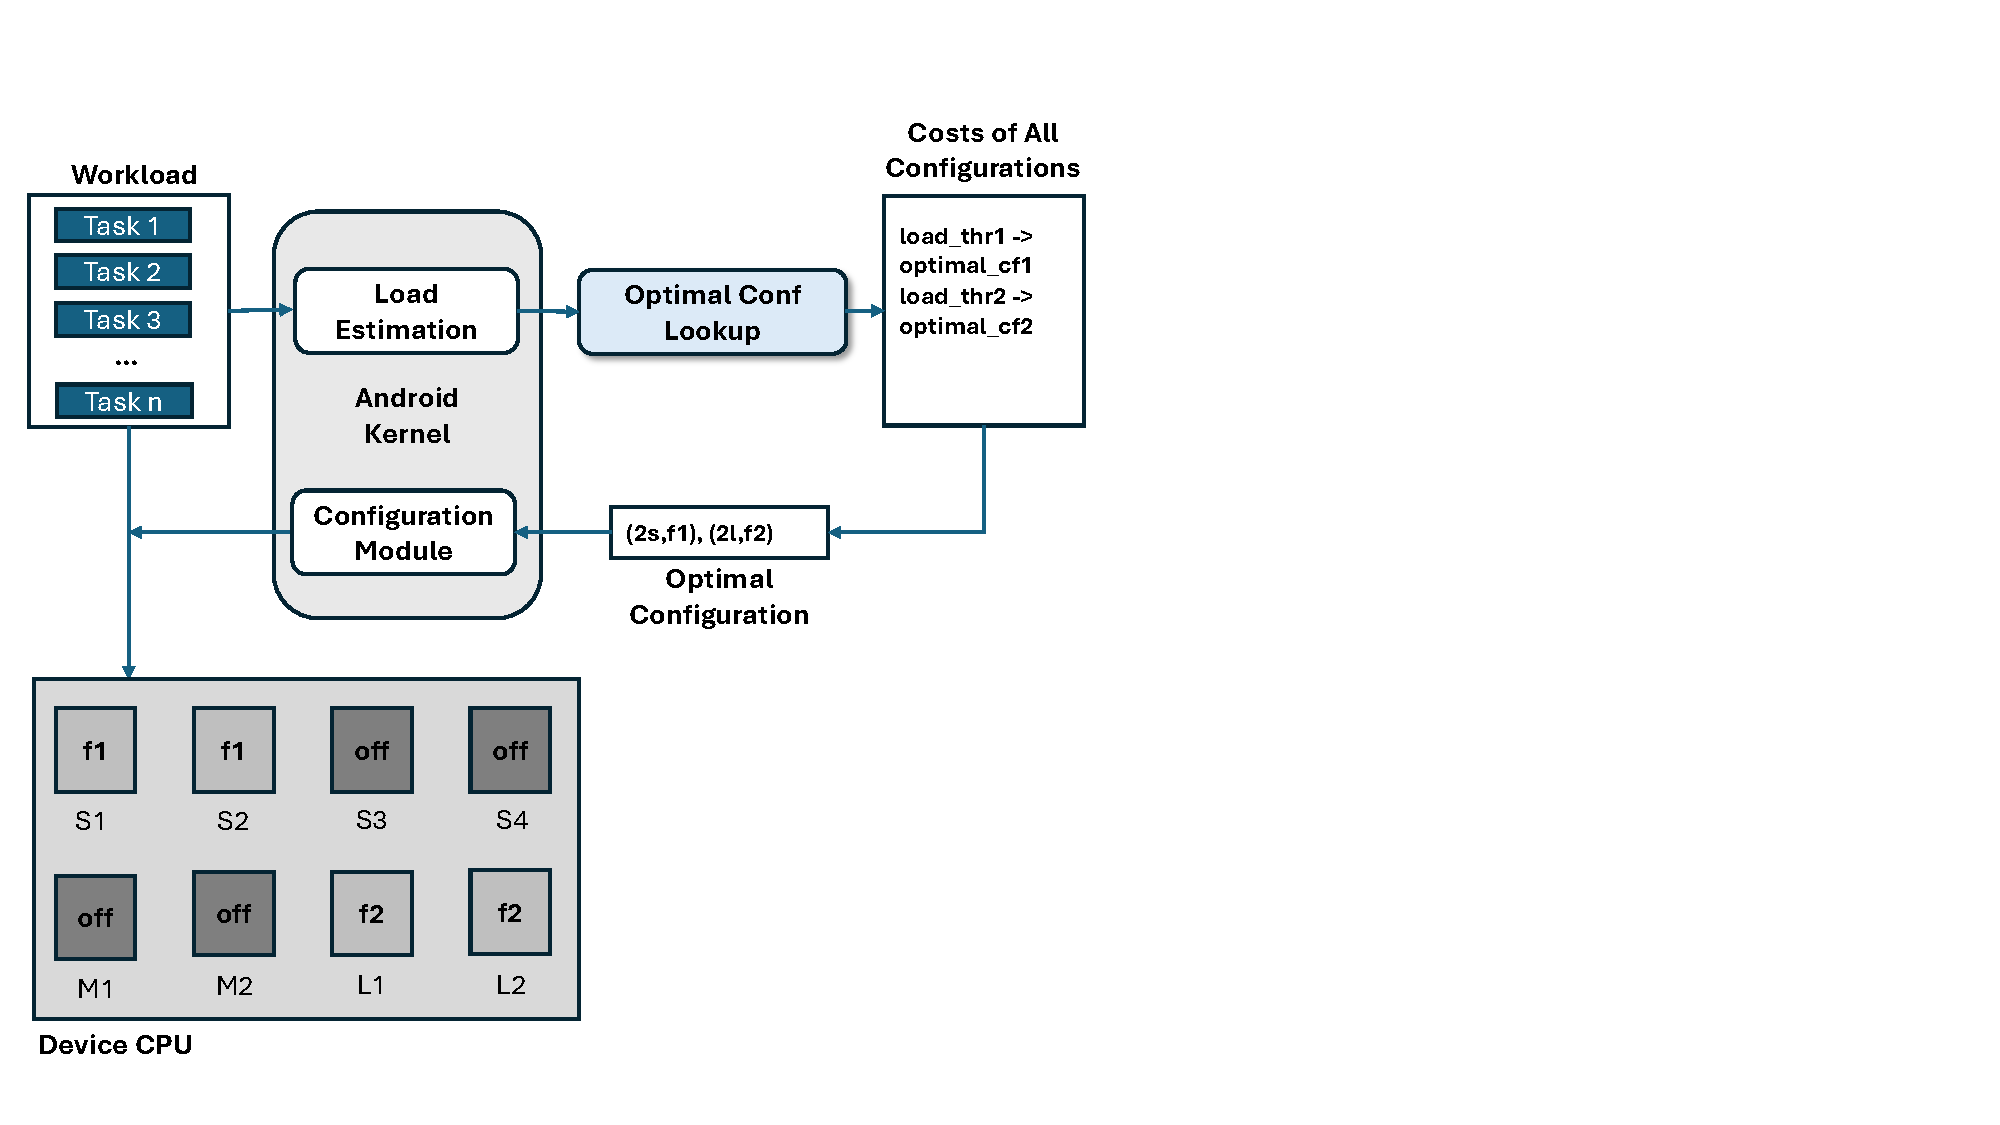
\includegraphics[scale=0.6]{ims/EuroPar2024Tool.pdf}
\end{center}
\caption{Optimal CPU configuration workload.}
%\caption{Our energy efficient scheduling workflow: the workload of the system, comprising a number of tasks, is analysed and the load of the system is estimated. This estimation is passed through the regression model, which estimates the cost (in terms of performance and energy consumption) of executing the workload under every possible CPU configuration, where a configuration denotes all the cores that are switched on and their frequencies. For example, the configuration (2s, fr1, fr2) is the configuration where two small cores are switched on, and they operate on frequencies fr1 and fr2. The list of estimated costs for each configuration is then passed to the configuration selector, which selects an optimal configuration. This configuration is then passed to the configuration module, which is a part of the Android kernel that switches off the cores that are not to be used (by preventing any tasks being scheduled on them) and sets the appropriate frequency of the ones that should be kept on. This whole process is repeated periodically (by default, every 100ms).}
%\caption{Optimal CPU configuration workload.}
\label{fig:workflow}
\end{figure*}


Our approach for deriving energy-optimal CPU configurations for Android workloads is the following. Given a workload (consisting of the threads of currently running applications), we characterise the workload by a number between 0 and 1, describing the overall utilisation of a full system. Based on this overall utilisation we decide which processor cores in the system will be powered on and at what frequency they will operate. Our aim is to allocate as few cores as possible (leaving the remaining ones switched off) in order to preserve energy whilst also not decreasing the quality-of-service significantly. Our workflow is summarised in~\cref{fig:workflow}. Firstly, the workload of the system is profiled for its load characteristics, including the utilisation of the system (a percentage, between 0 and 1) and the total number of threads. After that, the lookup table of optimal (in terms of energy efficiency) CPU configurations for a given (range of) system loads is consulted, and the optimal CPU configuration is retrieved. The lookup table is created using a regression model, described in~\cref{sec:model}. For example, the configuration $(2s, f1),(2l, f2)$ is the configuration where two \emph{small} cores and two \emph{large} cores are switched on, with the \emph{small} cores operating at frequency $f1$ and the \emph{large} cores operating at frequency $f2$. The Android kernel configuration module then implements this configuration, switching off the cores that should not be used and setting the frequency of the remaining ones to the optimal ones, as specified in the lookup table. The implementation of this module is described in~\cref{sec:schedule}. The device then continues to operate with this configuration for a fixed time window (by default, 100ms), before repeating the process of estimating the system load and potentially selecting a new configuration.

\subsection{Modelling Energy Consumption for Android} \label{sec:model}

%670000 configurations

Taking into account all of the options for tuning the cores of an asymmetric mobile device processor (i.e. powering on and off individual cores and, for our example system, choosing between 11-20 different frequency options for each group of active cores), it is clear that deriving the optimal processor configuration for a given workload might involve searching through a large possible configuration space, which is impractical to be explored exhaustively. For our example system, there are $670,000$ possible configurations. To build a fully accurate lookup table, we would need to profile, for each range of system loads, the energy consumption and performance of each of the configurations, which is intractable.  

In order to determine the best configuration for a given workload, we use machine learning to build a power-performance model of the system. Our approach is illustrated in~\cref{fig:reg2}. First, we have created a synthetic benchmark that simulates a realistic workload of a system. The benchmark comprises a tight loop of non-memory instructions with the number of iterations per second taken as a proxy for per-core performance during the test. %\CB{Perhaps summarise them in a table}. 
We estimate system utilisation by considering the ratio of the predicted performance score (defined as the predicted number of total loop iterations per second) to the maximum observed performance score. We then select a subset of the possible processor configurations and run the benchmark on each of these configurations, recording its performance (in terms of the number of instructions executed) and energy consumption. These measurements are then used as training data for a regression model. The regression model takes as inputs the processor configuration (i.e. cores that are switched on and at what frequency they are operating) and returns the performance and energy consumption of the benchmark under that configuration. The regression model produces a table of performance and energy consumption for each of the $670,000$ configurations. The performance is then normalised by dividing it with the maximum performance with all the cores on, effectively giving us the system utilisation that can be achieved with the given configuration. As a final step, we divide all the possible system utilisations in the system utilisation ranges, and, for each system utilisation range, we compare the energy consumption across all configurations and select the configuration that achieves the minimum energy consumption. This gives us a table of \emph{(util\_range, conf)} pairs, where the \emph{conf} is the best (in terms of energy consumption) configuration that can handle the system loads in the \emph{util\_range} range. This is used as a runtime lookup table from which, depending on the current system load, we select the optimal processor configuration. 

%We illustrate our technique in Figure~\ref{fig:reg2}. An android devices is generally made up of an asymmetric device comprising a number of \emph{small} (denoted S), \emph{medium} (denoted M) and \emph{large} (denoted L) cores (as previously discussed in Section~\ref{sec:energyschedule}). Furthermore, a number of different configurations of these cores, in terms of which of the small, medium or large cores are powered on and off, and at which frequency, may be selected by the scheduler during the operation of the device. In order to build our regression model, and ultimately select which configuration is best to use during the operation of the device, we first execute a \emph{synthetic benchmark} for a number of configurations of the device. 
%(\CB{how many?}). 
%The synthetic benchmark is designed to draw the maximum the CPU cycles for the duration of the benchmark run in order to profile the limits of the performance and power draw for each configuration. The result of this is a table of configurations mapped to their performance and energy characteristics for the workload synthesised by the benchmark. These configurations are then fed into a regression model, which then predicts the performance and energy characteristics for \emph{all} possible configurations. On an Android Pixel 6a device, this complete configuration space is 670000 configurations. These 670000 configurations are then filtered by a \emph{Configuration Selector}, which selects the best configurations based on their energy characteristics, while discarding configurations that do not optimise for energy. For example, given the choice of two configurations, where \emph{Configuration 1} yields 100 ms of performance and 80 J of energy, and \emph{Configuration 2} yields 120 ms of performance and 70 J of energy, our selector would choose the second configuration with the reduced energy consumption, despite it yielding a slightly worse performance. The scheduler can then reconfigure the device using this selected configuration, based on the current workload of the device while the applications are running. This allows dynamic configuration of the device to match its changing workload characteristics in real time with minimal overhead.


\begin{figure*}[ht]
\begin{center}
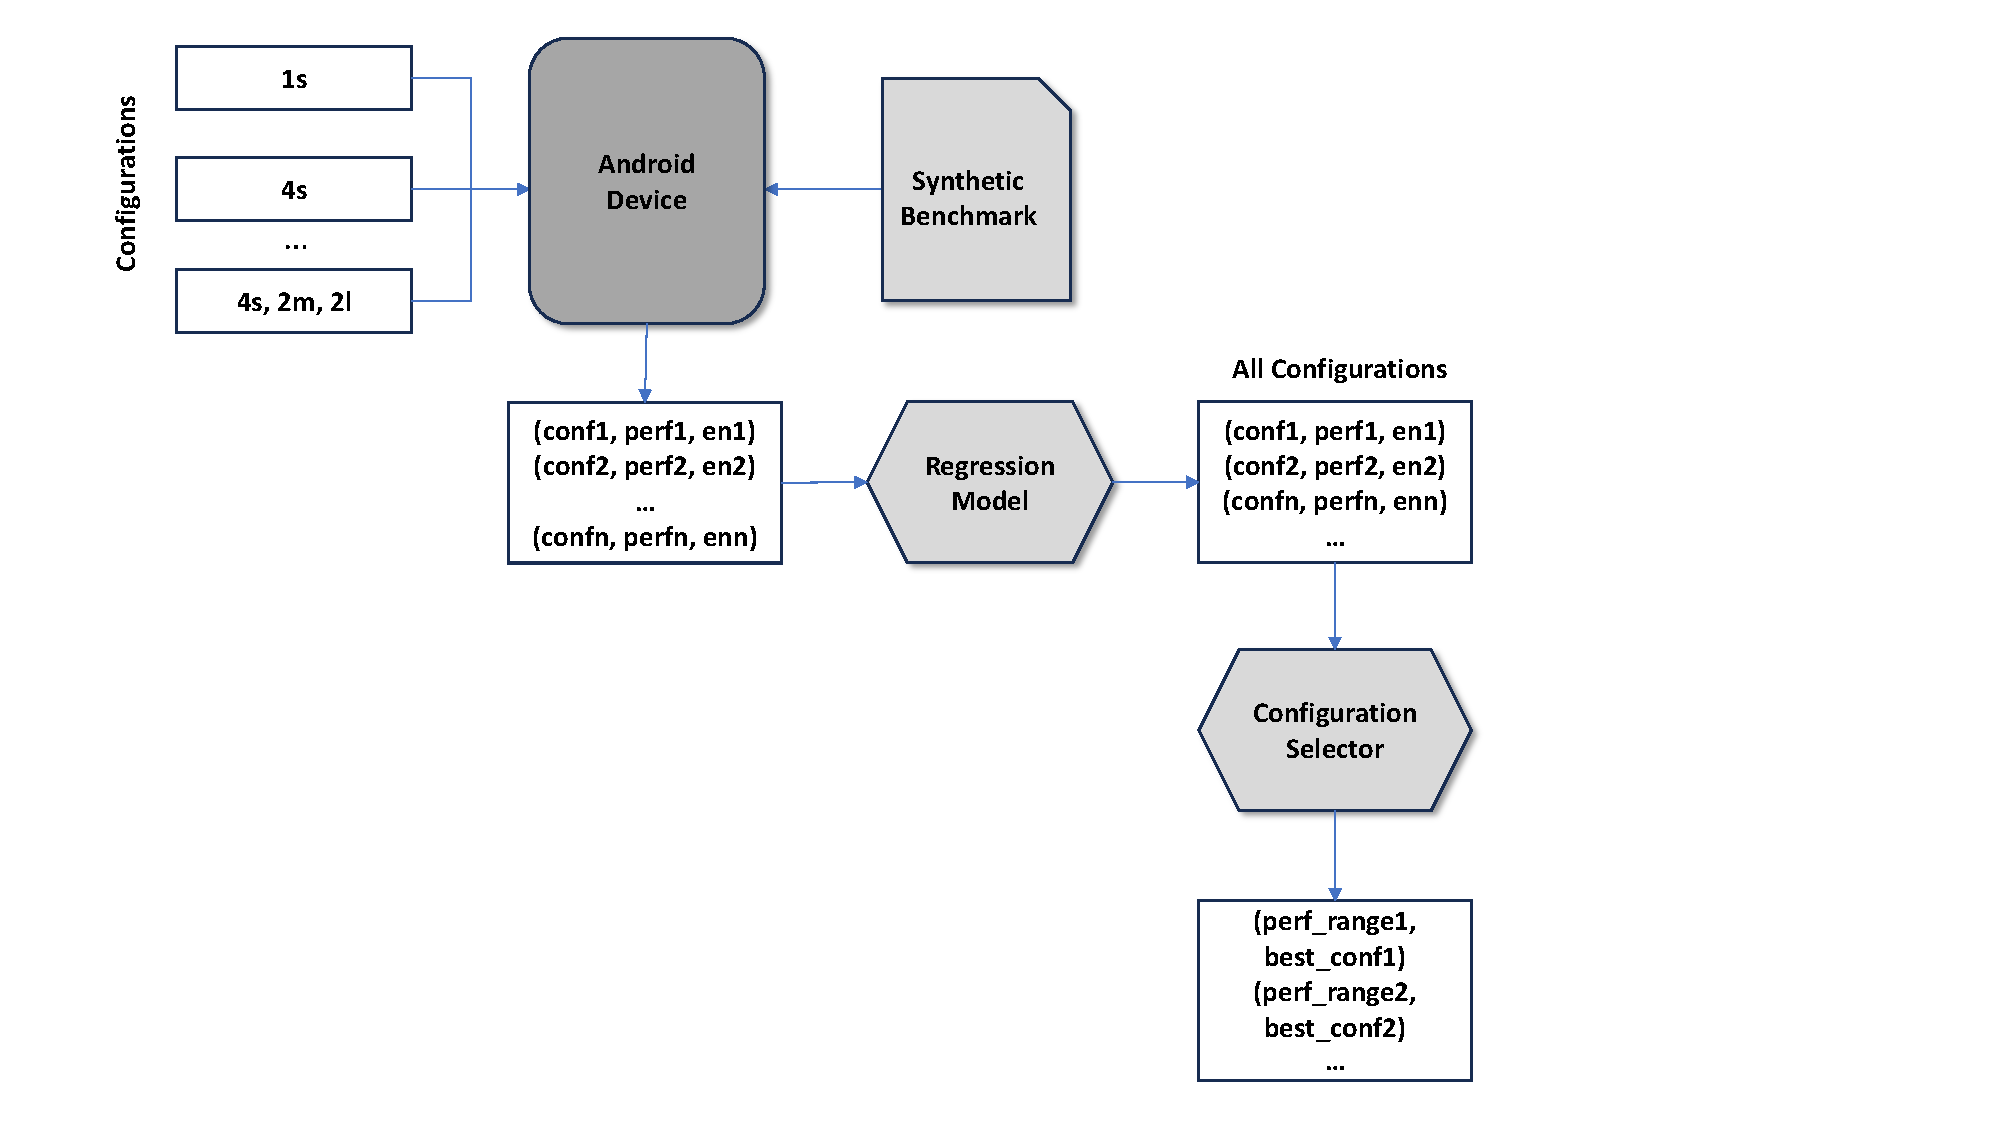
\includegraphics[scale=0.5]{ims/RegressionPaper.pdf}
\end{center}
%\caption{Our configuration selector workflow. A number of configurations of cores (e.g. small, medium and large) are profiled against a synthetic benchmark, resulting in a characterisation of the configurations against their performance and energy profiles. We then use a regression model over these configurations to predict the entire space of performance and energy metrics for the entire space of configurations that are available on the device. A Configuration Selector then determines from these which is the best configuration to use given the current workload of the system as it is running.}  
\caption{Workflow for deriving a table of the best processor configurations for a given system load.}
\label{fig:reg2}
\end{figure*}

%\CB{Need to give or summarise model}

\subsection{An Android Scheduler for Energy Efficient Computation} \label{sec:schedule}
% 3 pages
% psuedo code

Our power-performance model, described in~\cref{sec:model}, returns, for each system load, a predicted best processor configuration for that load. At runtime, the workload is computed by the Android kernel by weighting the on-time of each core against a vendor supplied table of scaling factors for each core/frequency pairing. This allows us to select the lowest-power state that still achieves enough performance for the current system workload.

Our technique for selecting the best processor configuration is implemented through kernel patches that periodically (e.g. once every 100 milliseconds) estimate the system workload, and selects the best configuration using our model and applies this configuration by turning the cores on or off and selecting their frequencies. Since selecting the best configuration is a simple lookup operation into a table, the overheads of selecting the best configuration are minimal. This allows dynamic configuration of the device to match its changing workload characteristics in real time with minimal overhead. One adjustment made to the algorithm was to include two measures of utilisation in the pre-computed tables: maximum single core performance in a given configuration, and total performance of all cores. The tweaked scheduler then selects the lowest power configuration that is able to provide enough single threaded performance for the most demanding active task and enough total system performance for all tasks currently running on the system. 

%We illustrate our technique in Figure~\ref{fig:reg2}. An android devices is generally made up of an asymmetric device comprising a number of \emph{small} (denoted S), \emph{medium} (denoted M) and \emph{large} (denoted L) cores (as previously discussed in Section~\ref{sec:energyschedule}). Furthermore, a number of different configurations of these cores, in terms of which of the small, medium or large cores are powered on and off, and at which frequency, may be selected by the scheduler during the operation of the device. In order to build our regression model, and ultimately select which configuration is best to use during the operation of the device, we first execute a \emph{synthetic benchmark} for a number of configurations of the device. 
%(\CB{how many?}). 
%The synthetic benchmark is designed to draw the maximum the CPU cycles for the duration of the benchmark run in order to profile the limits of the performance and power draw for each configuration. The result of this is a table of configurations mapped to their performance and energy characteristics for the workload synthesised by the benchmark. These configurations are then fed into a regression model, which then predicts the performance and energy characteristics for \emph{all} possible configurations. On an Android Pixel 6a device, this complete configuration space is 670000 configurations. These 670000 configurations are then filtered by a \emph{Configuration Selector}, which selects the best configurations based on their energy characteristics, while discarding configurations that do not optimise for energy. For example, given the choice of two configurations, where \emph{Configuration 1} yields 100 ms of performance and 80 J of energy, and \emph{Configuration 2} yields 120 ms of performance and 70 J of energy, our selector would choose the second configuration with the reduced energy consumption, despite it yielding a slightly worse performance. The scheduler can then reconfigure the device using this selected configuration, based on the current workload of the device while the applications are running. This allows dynamic configuration of the device to match its changing workload characteristics in real time with minimal overhead.

%\CB{Perhaps give an example schedule derived?}

\section{Evaluation}

%%\begin{table}[ht]
%%\centering
%%\resizebox{10cm}{!}{%
%%\begin{tabular}{|c|c|}
%%\hline \hline
%%\textbf{Category} & \textbf{Pixel 6a} \\ % & \textbf{Pixel 7} \\
%%\hline
%%      OS version & Android 13/Lineage OS 1.20 \\
%%      Kernel version & Linux version 5.10.157-g69987828e43a \\
%%      Architecture & AArch64 \\
%%      Endianness & Little endian \\
%%      Number of CPUs & 8  \\
%%      CPU frequencies & \makecell {4x1.8GHz \\ 2x2.25GHz \\ 2x2.8GHz} \\
%%      RAM & 6GB  \\
%%      \hline \hline
%%\end{tabular}
%%}
%%\caption{Device and OS specifications for the Android mobile device used for the evaluation results.}
%%\label{tab:devicespecs}
%%\end{table}

In this section we evaluate our regression model and configuration selector from~\cref{sec:energyschedule} on a number of scenarios for Android that are designed to simulate realistic workloads and usage. These scenarios are described in~\cref{sec:scenarios}. We evaluate our scheduler over these scenarios on a Pixel 6a device (given in~\cref{tab:devicespecs}), comparing the energy savings from our energy-efficient scheduler against the default Android scheduler%, including the battery saving mode. 
We also measure the Quality of Service achieved for each scenario to check that we are sacrificing quality of service too much in gaining energy efficiency. We first describe our techniques for measuring energy and Quality of Service in~\cref{sec:measureeneryqos}, and then give results in~\cref{sec:scenarios}.


\subsection{Measuring Energy and Quality of Service} \label{sec:measureeneryqos}


The Pixel 6a device features Samsung \emph{s2mpg10} and \emph{s2mpg11} power supply chips. These provide the main voltage rails used on the device and have internal current and voltage sensors. The ICs can be configured to integrate and report total energy for a user-controlled subset of the rails via their I$^2$C interfaces. For this work we used these reported energy values, which are not affected by the presence of external power or the current charge/health of the device's battery.

Our technique relies on intentionally reducing the performance of the device in situations where it is not required. Therefore, direct measurements of CPU performance are not suitable for evaluating the technique. As an appropriate proxy for the end-user's experience using the device, we instead opted to use Android's notion of \emph{janky} UI frames. These measure the number of dropped frames that failed to be rendered and presented to the display within the required time limit, leading to a subjective experience of a stuttering and lagging device. We capture the cumulative number of \emph{janky} frames before and after each run and compute the total number of \emph{janky} frames per second, the total number of \emph{non-janky} frames per second, and the percentage of rendered frames that were \emph{janky}.

\subsection{Use Case Scenarios and Results} \label{sec:scenarios}
We evaluate our technique over five use case scenarios, representing a realistic use of mobile phones by typical users. Our goal was to test our processor configuration method on these scenarios and to achieve measurable improvements in energy consumption. The considered scenarios, all of which are available as C++ programs at https://github.com/yalmalaq/scenarios, are:
%XX \CB{need a public repo}

%\begin{enumerate}
 %   \item Description of the use-case:
    \begin{itemize}
    
\item \textbf{Social Media}: This scenario models the foreground use of two well-known social media applications, Twitter (X) and TikTok. The benchmark starts by opening the X app and navigating the tweets in the timeline for one minute. Then, a new tweet is created, after which the TikTok app is opened and videos from it are played for one more minute.

\item \textbf{Web browsing}: This scenario models web browsing, including reading text and watching videos from websites. The web browser app is started, and different websites are loaded, each for 30 seconds (BBC, Daily Mail, Vice and Reddit). On each website, we simulate slow scrolling up and down on the screen, to simulate the user activity.

\item \textbf{Game Playing:} This scenario models playing video games. The game app is called OfflineGames, which offers many games. One of the games that requires movement and touch on the screen is picked, and then automatically played for 2 minutes.

\item \textbf{Background Music}: This scenario models playing random music in the background of the mobile for 2 minutes, using the SoundCloud application. 

\item \textbf{Video Call:} This scenario makes a video call using the Microsoft Teams app. The call lasts for 2 minutes.

\item \textbf{Idle:} In this benchmark, no user applications are running in the foreground. All that is running are background system tasks. 
\end{itemize}

%\item 
\noindent
%Results: This part discusses the results of the energy and power consumption data obtained after executing the benchmarks of android application scenarios across ten samples using all 8 cores. It is clear that there were varying degrees of percentage decreases in most of the benchmarks in battery saver mode compared to the baseline. For instance, the significant impact of the battery saver on power consumption was on the Idle benchmark of approximately 37.28\%. Social media comes after in terms of a percentage change of about 27\%. Whereas the power result in the battery saver and the baseline setting were quite similar for the Web browsing and Video call benchmarks. Energy, in contrast, shows Idle and Social media benchmarks showing the highest percentage of energy savings of about 26\%. A slight impact was shown in background music and video playing of about 2.6\% and 8\%, respectively. However, the web browsing benchmark indicates the baseline setting outperforms the battery saver by around 15.89\%.

\noindent
\cref{tab:usecase} shows our preliminary results so far obtained on the Pixel 6a device, where we only report evaluation figures for three of the benchmarks (idle, social media and web) due to unforeseen crashing in the execution. The idle benchmark performs slightly worse in terms of energy with our technique, reporting 27 J of energy instead of 25 J in the baseline case. The frames-per-second (FPS) and the Janky frames can not be measured for the idle application. For social media, our technique performs much better, with 59.61 J of energy vs. 117.72 J in the baseline case, a 50.62\% decrease in energy consumption. Unfortunately, however, the QoS drops, from 44 FPS and 0.7 Janky frames in the basecase, to 12 FPS and 88.9 Janky frams for our technique. Finally the web application performs better too: 54 J of energy consumption vs. 169 J of energy consumption in the baseline case, a 68\% reduction in energy consumption. Again, however, the QoS drops, from 30 FPS to 10 FPS and 1.34 Janky frames to 85 Janky frames. We believe the drops in QoS are due to an over agresssive selection filter being applied. We intend to tune this selection figure and fix the crashing issues for the final submission of the paper. 


  
%\end{enumerate}

%  \begin{table}
% \begin{center}
% \resizebox{12cm}{!}{%
%   \begin{tabular}{|c|c|c|c|c|c|c|c|c|}
%     \hline
%     \multirow{4}{*}{Benchmark} & \multicolumn{8}{c|}{Energy (J)} \\
%     \cline{2-9}
%      & \multicolumn{2}{c|}{Baseline} & \multicolumn{2}{c|}{Battery Saver} & change & \multicolumn{2}{c|}{methodXX} & change \\
%     \cline{2-9}
%     & mean & std & mean & std & \% & mean & std & \%\\
%     \hline
%     Background music & 104.88&11.63 &102.12 &13.33 & -2.63\% & XX & XX & XX \\
%     \hline
%      Video playing &198.72 &17.45 &182.16 & 14.25 &-8.33\%& XX & XX & XX\\
%     \hline
%      Social media  &234.60 &14.55 &171.12 & 11.642 &-27.06\% & XX & XX & XX\\
%     \hline
%      Web browsing  & 295.32 &13.33 &342.24 & 14.25  &15.89\% & XX & XX & XX\\
%     \hline
%      Video call &408.48 &11.634 &405.72 &13.33  &-0.67\% & XX & XX & XX\\
%     \hline
%     Idle &77.28 &21.77& 57.96 & 8.73 & -25.00\% & XX & XX  & XX\\
%     \hline
 
%   \end{tabular}
% }
%   \caption{Standard deviation and mean values of baseline compared with a battery saver using 8 cores across 10 runs.}
%   \label{tab:usecase}
%  \end{center}
% \end{table}

% \begin{table}
%\begin{center}
%\resizebox{12cm}{!}{%
%  \begin{tabular}{|c|c|c|c|c|c|}
%    \hline
%    \multirow{4}{*}{Benchmark} & \multicolumn{5}{c|}{Energy (J)} \\
%    
%     & \multicolumn{2}{c|}{Baseline} & \multicolumn{2}{c|}{methodXX} & change \\
%    
%    & mean & mean & fps & jank \%\\
%    \hline
%    Background music & 104.88 & 11.63 & XX & XX & XX \\
%    \hline
%     Video playing &198.72 &17.45 & XX & XX & XX\\
%    \hline
%     Social media  &234.60 &14.55 & XX & XX & XX\\
%    \hline
%     Web browsing  & 295.32 &13.33 & XX & XX & XX\\
%    \hline
%     Video call &408.48 &11.634 & XX & XX & XX\\
%    \hline
%    Idle &77.28 &21.77 & XX & XX  & XX\\
%    \hline
% 
%  \end{tabular}
%}
%  \caption{Standard deviation and mean values of baseline compared with our technique using 8 %cores across 10 runs.}
%  \label{tab:usecase}
% \end{center}
%\end{table}

\begin{table*}
\renewcommand{\arraystretch}{1.3}
\caption{mean values of baseline compared with our technique using 8 cores across 10 runs.}
\label{tab:usecase}
\centering
%\resizebox{12cm}{!}{
\begin{tabular}{|c|c|c|c|c|c|c|}
\hline
\textbf{Benchmark} & \textbf{Base Energy} & \textbf{Our Energy} &  \textbf{Base FPS} & \textbf{Our FPS} & \textbf{Base Janky} & \textbf{Our Janky} \\
\hline
      Idle &  25.35 J &  27 J  & N/A & N/A & N/A & N/A \\ 
      Social Media & 117.74 J & 59.61 J & 44 & 12 & 0.7 & 88.9 \\
      Web & 169 J & 54 J & 30.7 & 10.35 & 1.34 & 85.68 \\
     % 4S & 730 J & \textbf{-9.75\%} & 1.58 JFPS & \textbf{170.5\%} \\
     % 4S + 2M & 721 J & \textbf{-10.86\%} & 0.56 JFPS & \textbf{-3.9\%}\\
     % 4S + 2L & 1057 J &  \textbf{30.717\%} & 0.54 JFPS & \textbf{-6.8\%}\\
     % Our system & X J &  \textbf{X\%} & X & \textbf{X\%}\\
      \hline
\end{tabular}
%}

\end{table*}



\begin{table*}
\renewcommand{\arraystretch}{1.3}
\caption{Energy Consumption and Quality of Service of the Social Media Scenario Under Different CPU Configurations}
\label{tab:energymusic}
\centering
\begin{tabular}{|c|c|c|c|c|c|}
\hline
\textbf{Cores on} & \textbf{Energy} & \textbf{Energy Diff} &  \textbf{QoS} & \textbf{QoS Diff} \\
\hline
      All &  809 J &     \textbf{0\%}  & 0.58 JankyFPS & \textbf{0\%} \\ 
      1S & 737 J & \textbf{-8.79\%} & 3.47 JFPS & \textbf{494.0\%} \\
      2S & 757 J & \textbf{-6.39\%} & 4.70 JFPS & \textbf{705.1\%} \\
      4S & 730 J & \textbf{-9.75\%} & 1.58 JFPS & \textbf{170.5\%} \\
      4S + 2M & 721 J & \textbf{-10.86\%} & 0.56 JFPS & \textbf{-3.9\%}\\
      4S + 2L & 1057 J &  \textbf{30.717\%} & 0.54 JFPS & \textbf{-6.8\%}\\
  %  Our system & X J &  \textbf{X\%} & X & \textbf{X\%}\\
      
      \hline
\end{tabular}
\end{table*}



\section{Related Work} \label{sec:relatedwork}

%\begin{itemize}
% \item comprof, complace \cite{comprof}
% \item teamplay stuff \cite{teamplay} \cite{CSL-Types} \cite{CSL}
%\item ``Energy Efficient Scheduling'' - review of algorithmic techniques for energy conservation in big data sets. \cite{Albers2022}
%\item EA-DFPSO: An intelligent energy-efficient scheduling algorithm for mobile edge networks \cite{LU2022237}
% \item Towards an Operating System Based Framework for
%Energy-Efficient Scheduling of Parallel Workloads 
%\item Energy-Efficient Load Balancing Algorithm for Workflow Scheduling in Cloud Data Centers Using Queuing and Thresholds 
%\item Yasir's thesis? \cite{yasir}
%\item Energy-Efficient Scheduling for Multi-Core Processors \cite{lieder08energy-efficient-scheduling}
%\item Linux kernel docs: \footnote{https://docs.kernel.org/scheduler/sched-energy.html}
%\item Energy-Efficient Soft Real-Time CPU Scheduling for
%Mobile Multimedia Systems \cite{wanghong}
%\item Optimizing Energy Consumption of Mobile Games \cite{Yonghun}
%\item Who killed my battery?: Analyzing mobile browser energy consumption \cite{narendran}
%\item AppScope: Application energy metering framework for android smartphone using kernel activity monitoring \cite{Yoon}
%\item Toward energy-aware balancing of mobile graphics \cite{10.1117/12.2079602}
%\item Scheduling for reduced CPU energy \cite{Weiser1996}
%\end{itemize}

There has been relatively little work in the area of scheduling to reduce energy efficiency on mobile devices. Energy efficient scheduling for CPUs, however, dates back to the 1990s, with work by Weiser et al.~\cite{Weiser1996}, and the Linux scheduler has some limited Energy Aware Scheduling\footnote{https://docs.kernel.org/scheduler/sched-energy.html}. \cite{Albers2022} gives a review of various algorithmic techniques for energy conservation in processing big data sets, and Lv~\cite{lv} gives a study of energy-efficient scheduling using dynamic voltage and frequency scaling. These reviews includes dynamic speed scaling and power-down mechanisms where idle devices can be transitioned to idle devices and are not focused on mobile device scheduling. In~\cite{LU2022237} Lu et al. propose ``Energy-aware Double-fitness Particle Swarm Optimization'' (EA-DFPSO) that employs swarm optimisation algorithms for achieving energy efficiency in edge computing environments. Malik et al propose a technique for Cloud computing using Particle Swarm Optimisation in~\cite{malik}. For parallel workloads, Shankar et al.~\cite{shankartowards} proposes a scheduling technique for multicore power monitors, management and control via power-aware task scheduling and load balancing.  

In~\cite{comprof}, the authors present COMPROF and COMPLACE,
a profiling tool and thread placement technique for shared-
memory architectures. COMPROF and COMPLACE that uses dynamic binary instrumentation to intercept memory operations and estimate inter-thread communication overhead, deriving (and possibly visualising) a communication graph of data-sharing between threads. This graph is then used to provide an optimal placement of threads, minimising communication latency. COMPROF demonstrates energy savings of up to 10\%.

The EU Teamplay project~\cite{teamplay} provided various techniques for helping software developers with writing energy efficient code. Amongst these techniques included the Contract Specification Language (CSL)~\cite{CSL}, a Domain Specific Language and contract system~\cite{CSL-Types} in C for expressing Time and Energy budgets for embedded devices. The authors also proposed~\cite{Jadhav:2019:JRWRTC} a technique using compiler intrinsics via a DSL entitled REEL, to allow users to express non-functional requirements; the compiler then performs ILP-based optimisation. Finally, Alguwaifli in~\cite{yasir} proposed a system using a combination of regression analysis and meta-heuristics to predict energy consumption over multiple X86 core frequencies for a variety of languages, including Haskell and C++.

There have been various techniques for reducing energy consumption on Android devices, mostly employing frequency scaling. AppScope~\cite{Yoon} provides a kernel module that uses event-driven monitoring to estimate energy consumption of Android applications, but does not offer more efficient scheduling for energy efficiency. GRACE-OS~\cite{wanghong} offers a mobile kernel providing a soft real-time scheduler. GRACE-OS attempts to balance QoS with more efficient energy consumption of mobile applications, using CPU speed scaling and Dynamic Voltage Scaling. Unlike the approach presented in this paper, GRACE-OS seems to work well for small-loaded systems and favours low frequency CPU scaling. In~\cite{narendran}, Thiagarajan et al. introduce a profiling technique for studying energy consumption of web browsing on mobile devices, allowing programmers to manually modify their web scripts to save energy. Stavrakis et al. present power measurements of running the Unity3D engine on a mobile device, and tuned the scene complexity parameters using a frequency scaling algorithm; this resulted in better energy efficiency of up to 40\%. However, unlike our approach, they do not consider general scheduling of android applications. Yonghun et al.~\cite{Yonghun} propose a technique for improving energy efficiency of video games on mobile devices. Finally, Janjic et al.~\cite{monte} employ a similar heuristic approach for searching the space of skeletal nestings and mappings for heterogeneous multi-core architectures, but employ a monte-carlo based search heuristic, rather than regression based techniques. 

\section{Conclusions and Future Work} \label{sec:conclusions}

In this paper we demonstrated a new technique for the dynamic scheduling of application workloads on mobile asymmetric multicore processors. Our technique is based on the dynamic assignment of optimal frequencies to groups of processing cores, based on a regression technique, which changes groups of cores on and off, in response to the changing of the system load. In this paper we targeted an Android Pixel 6a device, as a demonstration mobile platform. We evaluated our technique on a number of representative Android workloads, simulating real user activity through a number of applications such as video playing, social media, web browsing and video calling. Through our evaluation we were able to demonstrate an improvement in energy of up to 68\%.
%, while still preserving the Quality of Service of the device, with a maximum reduction in QoS of YY\% overall, compared to the Android default OS kernel scheduler. 

In the future, we plan to take the work in a number of new directions. We will firstly perform more experiments on other Android devices with other interesting asymmetric configurations. We will also look to target asymmetric multicore workloads in other settings, such as tablets and even desktop devices, scaling our technique to reduce energy on those devices too while still preserving the Quality of Service. We will also try different heuristic and machine-learning approaches and compare those against our regression approach.

\bibliographystyle{IEEEtran}
\bibliography{bib}


\end{document}
